%\setchapterimage{bandeau}
\chapter*{TD \arabic{cptTD} \\ 
Système d’ouverture et de fermeture de portes de tramway -- 
\ifprof Corrigé \else Sujet \fi}
\addcontentsline{toc}{section}{TD \arabic{cptTD} :
Système d’ouverture et de fermeture de portes de tramway -- 
\ifprof Corrigé \else Sujet \fi}

\iflivret \stepcounter{cptTD} \else
\ifprof  \stepcounter{cptTD} \else \fi
\fi

\setcounter{question}{0}
\marginnote{Centrale Supelec -- PSI -- 2008.}
\marginnote[1cm]{
\UPSTIcompetence[2]{C1-02}
\UPSTIcompetence[2]{C2-04}}

\begin{marginfigure}[4cm]
\centering
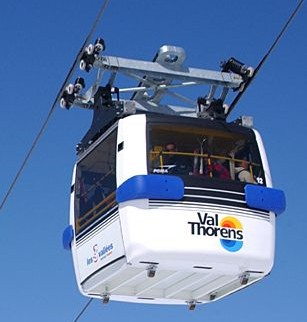
\includegraphics[width=\linewidth]{fig_00}
\end{marginfigure}

\subsection*{Présentation}

\subsection*{Étude du régulateur de la boucle de vitesse}

\begin{obj}Déterminer un régulateur de vitesse permettant d’atteindre les exigences
suivantes :
\begin{itemize}
\item écart nul en régime permanent pour une consigne de vitesse constante et un effort perturbateur, dû à la poussée des passagers, constant;
\item marge de phase $\Delta \varphi \geq 45\degres$ pour un modèle nominal qui sera précisé par la suite;
\item bande passante la plus grande possible compte tenu de la contrainte de marge de phase;
\item temps de réponse inférieur à \SI{0,2}{s} en réponse à une variation en échelon de l’effort perturbateur.
\end{itemize}
\end{obj}


\begin{marginfigure}
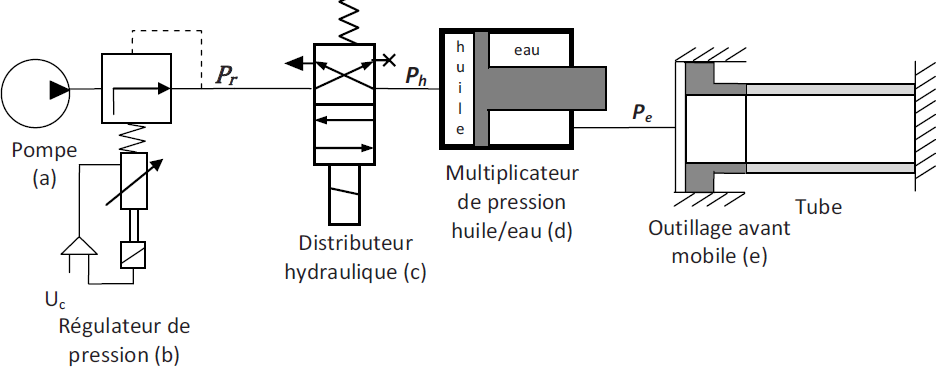
\includegraphics[width=\linewidth]{fig_01}
%%\textit{}
\end{marginfigure}

La chaîne de régulation de vitesse est décrite par le schéma-blocs suivant où la fonction de transfert représente la chaîne de mesure de vitesse comportant un filtre
du 1\ier ordre, de constante de temps $\tau_f = \SI{10}{ms}$, permettant de limiter
l’impact des bruits de mesure et $G$ est le gain de l’amplificateur de puissance
alimentant le moteur.

On choisit d’adopter pour cette chaîne un régulateur de type proportionnel-intégral
dont la fonction de transfert est : $R(p)=K_r\left(1+\dfrac{1}{T_i p}  \right)$.

\question{Au regard des exigences du cahier des charges, justifier le choix
de ce type de régulateur.}

On cherche d'abord à évaluer le temps de réponse vis-à-vis des perturbations. 

\question{Déterminer la fonction de transfert en boucle fermée $T(p)=\dfrac{\Omega_1(p)}{F_1(p)}$ entre les perturbations dues à la poussée des passagers et la vitesse du moteur, en fonction des différentes fonctions de transfert de la figure précédente.  Montrer que la réponse fréquentielle peut être approchée par la relation :}

$$
|| T\left(j \omega\right) || = 
|| H_2\left(j \omega\right) || \cdot 
\min \left(
||H_1\left(j \omega\right)||; 
\left|\left| \dfrac{1}{R\left(j \omega\right)GH_3\left(j \omega\right)}\right|\right|\right)
$$

$$
= || H_2\left(j \omega\right) || || M\left(j \omega\right) ||.
$$


Pour la suite, on adopte les modèles de commande simplifiés suivants : 
$$
H_1(p)=\dfrac{10}{p} \quad
H_2(p)=0,05 \quad
H_3(p)=\dfrac{0,1}{1+0,01 p}\quad
G=10.
$$

Afin de limiter le périmètre de l’étude, on adopte sans justification les
hypothèses suivantes : 
\begin{itemize}
\item $1/T_i < \SI{100}{rad.s^{-1}}$;
\item la situation considérée est celle de la figure suivante représentant le diagramme asymptotique de la fonction 
$
\left|\left|\dfrac{1}{R\left(j \omega\right)GH_3\left(j \omega\right)}\right|\right|_{\text{dB}}
$ où $20\log G_0 < 0$.
\end{itemize}

\begin{marginfigure}
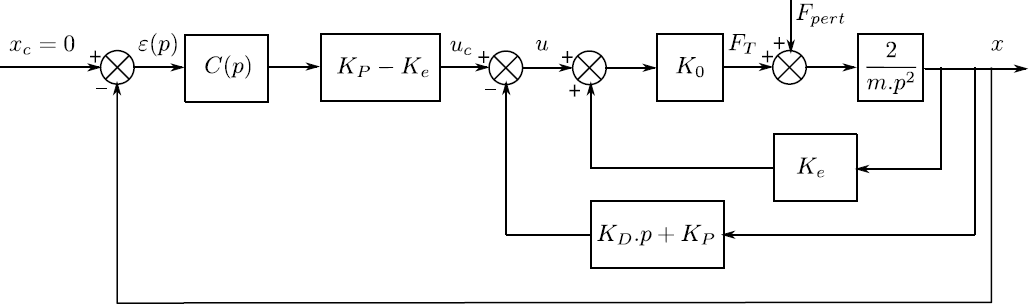
\includegraphics[width=\linewidth]{fig_02}
%%\textit{}
\end{marginfigure}

\question{Exprimer $G_0$ en fonction de $K_r$. En utilisant la figure précédente, tracer le diagramme asymptotique de la fonction $\left|\left|H_1\left(j \omega\right)\right|\right|$ (veiller
au respect des pentes) et celui de $\left|\left|M\left(j \omega\right)\right|\right|$ en adoptant l’approximation de la
question précédente.}

\question{En déduire alors une approximation de la fonction de transfert
$T(p)=\dfrac{\Omega_1(p)}{F_1(p)}$ en exprimant toutes les brisures en fonction de $K_r$ et $T_i$.}

\question{Proposer une nouvelle expression approchée de $T(p)$ sous la forme $T_a(p)=\dfrac{N(p)}{1+\tau p}$ où $N(p)$ est le numérateur de $T(p)$? En utilisant la forme approchée de $T_a(p)$, déterminer l'évolution de la vitesse $\Omega_1(t)$ en réponse à un échelon de la force de perturbation et tracer son allure. }

\question{En se référant à des fonctions types connues donner, en fonction de $T_i$, un ordre de grandeur du temps de réponse vis-à-vis de la force perturbatrice.}

\question{Justifier alors l’intérêt d’adopter pour $T_i$ la valeur la plus petite possible.}

\question{En vous aidant de tracés succincts de diagrammes
de Bode, analyser la stabilité du système
bouclé dans les deux cas : $\dfrac{1}{T_i}>\SI{100}{rad.s^{-1}}$ et $\dfrac{1}{T_i}<\SI{100}{rad.s^{-1}}$.}

\question{En prenant $K_r=1$, tracer les diagrammes
de Bode asymptotiques (module et phase) de la fonction de transfert en boucle
ouverte corrigée et l’allure de la courbe réelle du diagramme de phase. Veiller à
effectuer ce tracé de façon à respecter une situation stable du système en boucle
fermée.}

\question{En utilisant la représentation dans le plan de Bode donnée figure suivante, déterminer
quelle est la valeur $T_{i\text{min}}$ la plus petite possible que l’on peut conférer à $T_i$
compatible avec la marge de phase minimale exigée par le cahier des charges
(cette fonction servira uniquement à calculer en plaçant judicieusement
pour obtenir la marge de phase souhaitée).}


\begin{center}
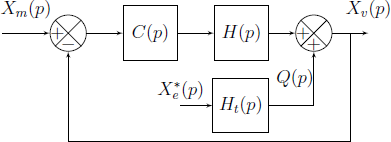
\includegraphics[width=\linewidth]{fig_03}
%%\textit{}
\end{center}

\question{En conservant la valeur $T_{i\text{min}}$ calculée précédemment, en déduire alors la
valeur du gain $K_r$ du régulateur permettant d’assurer la marge de phase souhaitée.}

\question{Vérifier si le cahier des charges est validé, et conclure sur l’adéquation
du régulateur calculé vis-à-vis du problème posé.}

